\documentclass[11pt,a4paper]{report}
\usepackage{graphicx,isabelle,isabellesym}

\usepackage[a4paper,includeheadfoot,margin=2.54cm]{geometry}

% further packages required for unusual symbols (see also
% isabellesym.sty), use only when needed

\usepackage{amssymb}
  %for \<leadsto>, \<box>, \<diamond>, \<sqsupset>, \<mho>, \<Join>,
  %\<lhd>, \<lesssim>, \<greatersim>, \<lessapprox>, \<greaterapprox>,
  %\<triangleq>, \<yen>, \<lozenge>

%\usepackage{eurosym}
  %for \<euro>

%\usepackage[only,bigsqcap]{stmaryrd}
  %for \<Sqinter>

%\usepackage{eufrak}
  %for \<AA> ... \<ZZ>, \<aa> ... \<zz> (also included in amssymb)

%\usepackage{textcomp}
  %for \<onequarter>, \<onehalf>, \<threequarters>, \<degree>, \<cent>,
  %\<currency>

% this should be the last package used
\usepackage{pdfsetup}

% urls in roman style, theory text in math-similar italics
\urlstyle{rm}
\isabellestyle{it}

% for uniform font size
%\renewcommand{\isastyle}{\isastyleminor}

\begin{document}

\title{MiniSail}
\author{Mark P. Wassell}
\maketitle

\begin{abstract}
MiniSail is a kernel language for Sail~\cite{Armstrong2019}, 
an instruction set architecture (ISA) specification language. 
Sail is an imperative language with a light-weight dependent type system similar to refinement type systems such as~\cite{Vazou2014}.
From an ISA specification, the Sail compiler can generate theorem prover code and C (or OCaml) to give an executable 
emulator for an architecture.
The idea behind MiniSail is to capture the key and novel features of Sail in terms of their syntax, 
typing rules and operational semantics,
and to confirm that they work together by proving progress and preservation lemmas. 
We use the Nominal2 library to handle binding.
\end{abstract}

\tableofcontents

% sane default for proof documents
\parindent 0pt\parskip 0.5ex

% generated text of all theories
\input{session}

\begin{center}
  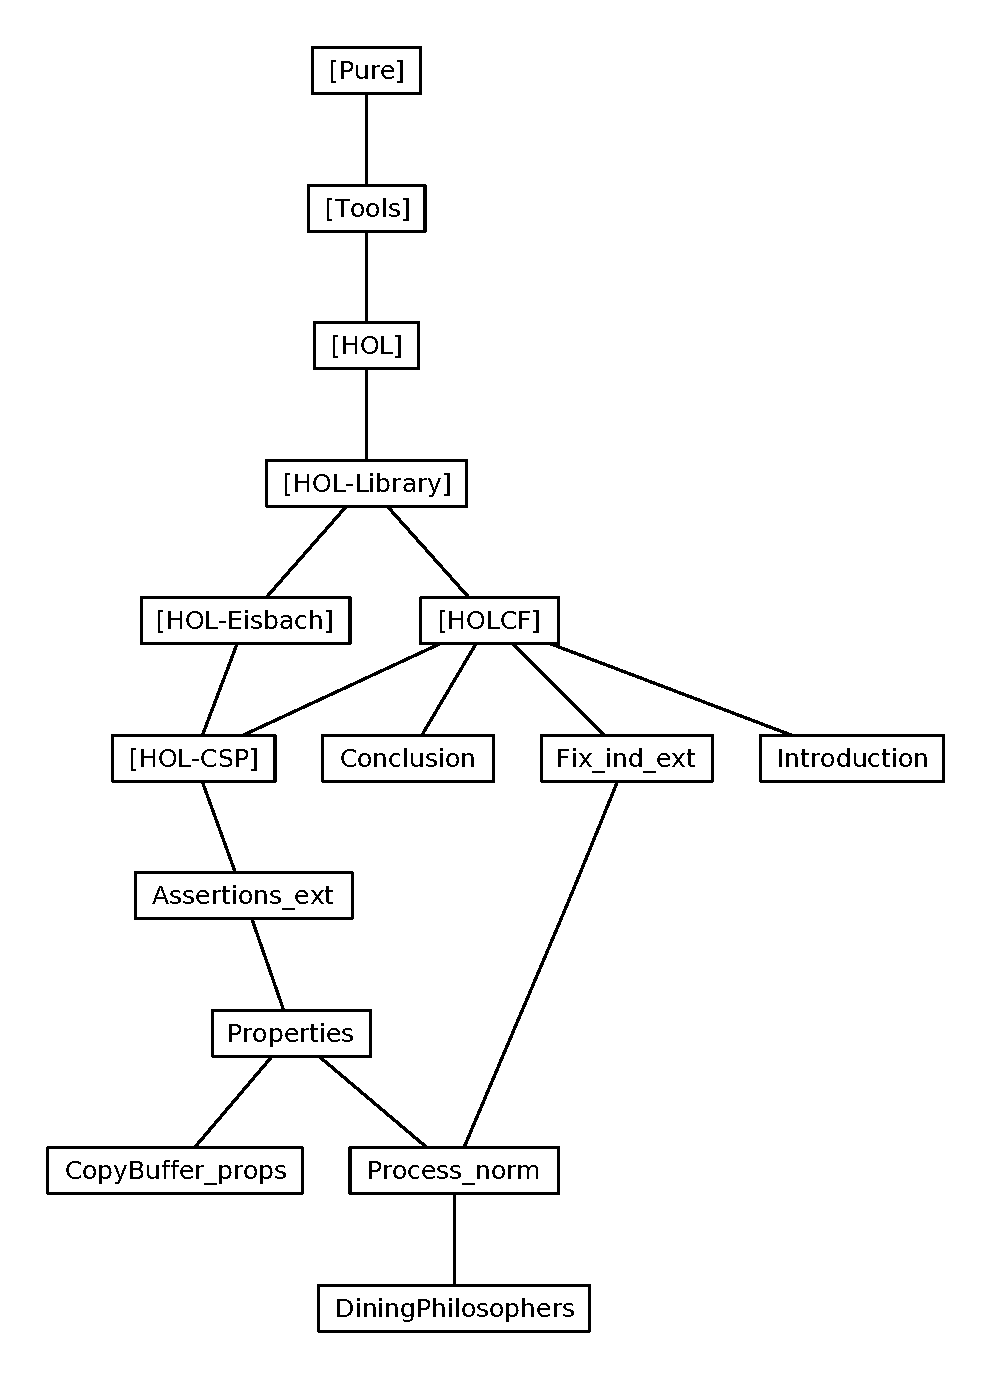
\includegraphics[width=\textwidth,height=\textheight,keepaspectratio]{session_graph}
\end{center}

\bibliographystyle{abbrv}
\bibliography{root}

\end{document}

